\section{Physical Implementation of Logical Operators}

Given an SPJM query, the selection, projection, and join operators are performed on relations and have the same physical implementations as those in relational databases.
The main difference lies in the physical implementation of matching operators.
In detail, if the graph-agnostic method in \refsec{solve-spjm-problem} is applied, the obtained logical matchings plans consist of selection, projection, and join operators.
Otherwise, if the graph-aware method is applied, the logical matching plans additionally include matching operators.
In this section, we focus on the physical implementions of the operators in logical matching plans.
Specifically, we focus on the join operators and matching operators in logical matching plans, because there can be many variations in the physical implementation of these two operators and the query performance varies greatly among different implementations. 

\begin{figure}
    \centering
    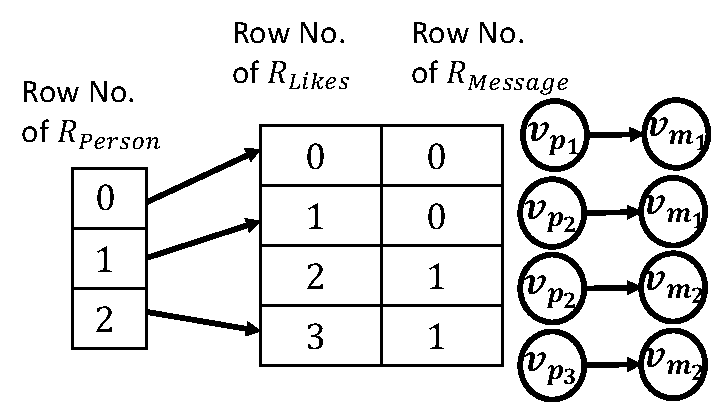
\includegraphics[width=.8\linewidth]{./figures/graph-index-likes.pdf}
    \caption{A Graph Index on edges labeled ``Likes'' on $G_1$ in \reffig{intro-rgmapping-example}.}
    \label{fig:graph-index}
\end{figure}

\subsection{Join Operators}
\label{sec:join-operator}
There are two kinds of join operators, where $\Join$ is defined over relations while $\widehat{\Join}$ is defined over graph relations.

For the first type of join operator (i.e., $\Join$), it is always utilized to ensure the adjacency relationships between vertices and edges.
For example, the join operator in $\relation{Person} \Join \relation{Likes}$ is used to ensure that the obtained edges labeled ``Likes'' are adjacent to vertices labeled ``Person''.

In a property graph, the adjacency relationships between vertices and edges are obvious and the adjacent edges of a vertex can be obtained directly.
Moreover, a tuple in a relation corresponds to a vertex or an edge in the property graph according to the \rgmapping.
Therefore, by maintaining the relationships between vertices and edges via indices, the join operation can be markedly accelerated. 
This improvement is achieved because for each tuple within a relation, the indices have pre-stored the tuples that are joinable with it. 
As a result, it eliminates the necessity to iterate through every tuple of the counterpart relation, thereby enhancing the efficiency of the join process.
As this index structure mimics the adjacency relationship between vertices and edges, it is called a graph index.


Specifically, a graph index is usually stored in a compressed sparse row (abbr.~CSR) \cite{} or adjacency matrix.
GrainDB \cite{graindb} introduces a graph index stored using CSR and an example is shown in \reffig{graph-index}.
In detail, the graph index is built on edges labeled ``Likes'' in property graph $G_1$ of \reffig{intro-rgmapping-example}(a) and records the adjacency relationships of the vertices labeled ``Person'' and the edges labeled ``Likes''.
That is, according to the \rgmapping, for each tuple $t_p$ in $\relation{Person}$, the tuples in $\relation{Likes}$ that can be joined with $t_p$ can be directly obtained with the graph index.

To elaborate, the first column of the index are row numbers in $\relation{Person}$ and row numbers start from 0.
For example, row number 1 represents the second tuple in $\relation{Person}$ with $person\_id = p_2$ (denoted by $t_{p_2}$) and this tuple corresponds to $v_{p_2}$ in $G_1$.
The second column records the row numbers in $\relation{Likes}$.
With this column, the edges adjacent to a given vertex can be retrieved efficiently.
For example, the edges adjacent to $v_{p_2}$ (i.e., $e_{l_2}$ and $e_{l_3}$ in $G_1$) are stored at row 1 and row 2 of $\relation{Likes}$.
It means that the second and third tuples in $\relation{Likes}$ can be joined with $t_{p_2}$.

If the adjacent relationships between vertices labeled ``Message'' and edges labeled ``Likes'' are also recorded in this index, the third column is added.
With this column, the neighbors of given vertices can be quickly accessed.
It means that given a tuple $t_p$ in $\relation{Person}$, let $T_{Likes}$ be the set of tuples in $\relation{Likes}$ which can be joined with $t_p$, and then the tuples in $\relation{Message}$ which can be joined with a tuple in $\relation{Likes}$ can be quickly obtained.
For example, the neighbors connected to $v_{p_2}$, connected through edges labeled ``Likes'', include $v_{m_1}$ and $v_{m_2}$, whose corresponding tuples are at row 0 and row 1 in $\relation{Message}$.
This information can be quickly ascertained through the graph index.


For the second type of join operator (i.e., $\widehat{\Join}$), if its right subtree is an matching operator $\matching(\pattern)$ whose pattern graph is a complete star, this join operator is denoted by $\widehat{\Join}_{ei}$ and implemented with extend-intersection.
Specifically, let \(\pattern = (v_r; \mathcal{H})\), $\mathcal{H} = \{v_1, \cdots, v_k\}, k \geq 2$, and denote the inputs of the join operator by $\relation{1}$ and $\relation{2}$, respective.
Then, an intuitive method to implement the join operator is as follows:
\begin{equation*}
    R_{1} \Join R_{\mathcal{L}(e_1)} \Join \cdots \Join R_{\mathcal{L}(e_k)} \Join R_{2},
\end{equation*}
where $e_x = (v_x, v_r), k \geq x \geq 1$.
However, in this process, the results must be instantiated once after each join is completed and numerous intermediate results are instantiated, significantly reducing query performance.

Please note that different edges (i.e., $e_1, \cdots, e_k$) intersect at the same vertex $v_r$.
Therefore, the intersection can be applied before the results are instantiated and fewer intermediate results are generated.
Then, the efficiency can be noticeably enhanced.

Moreover, if graph indices on $e_1, \cdots, e_k$ are available, the efficiency of the joins can be further improved by leveraging the graph indices to access joinable tuples quickly.


\subsection{Matching Operators}
\label{sec:matching-operator}
According to the graph-aware method, the matching operators in logical matching plans are all MMCs.
Specifically, based on different pattern graphs, MMCs in logical matching plans can be divided into two categories: 
(1) Matching Operators whose pattern graph is a complete star, denoted by $\matching_{star}$;
(2) Matching Operators whose pattern graph is an edge, denoted by $\matching_{edge}$.

For $\matching_{star}$, suppose its pattern graph is $\pattern = (v_r; \mathcal{H})$, it is implemented by scanning $\relation{\mathcal{L}(v_r)}$.

For $\matching_{edge}$, suppose the pattern is $(u_s) - [e] \rightarrow (u_t)$, then the matching operator is implemented by $\relation{\mathcal{L}(u_s)} \Join \relation{\mathcal{L}(e)} \Join \relation{\mathcal{L}(u_t)}$.
According to \refsec{join-operator}, if graph indices have been built on $\relation{\mathcal{L}(e)}$, these two joins can be implemented more efficiently by leveraging the graph indices.
Moreover, if there is no need to retain attributes on $e$ and there are no constraints on $e$, graph indices can be applied to get neighbors of $u_s$ directly without scanning $\relation{\mathcal{L}(e)}$.

